\documentclass[a0,final, portrait]{inriaposter}

\usepackage[utf8]{inputenc}
\usepackage[OT1]{fontenc}
\usepackage[english]{babel}
\usepackage{amsfonts, amsmath, amssymb, amsthm, dsfont, amsthm}
\usepackage{paralist}
\usepackage{wrapfig}

\usepackage{caption}
\usepackage{subcaption}

\usepackage{graphics}
\usepackage{graphicx}

\usepackage{epstopdf}

\providecommand{\mtx}[1]{\mathbf{#1}}

\begin{document}

\sffamily

\postertitle%
{Poppy: Open Source 3D Printed Robot for Experiments in Developmental Robotics}
{Matthieu Lapeyre, Pierre Rouanet, Jonathan Grizou, Steve N'Guyen, \\ Alexandre Le Falher, Fabien Depraetre, Pierre-Yves Oudeyer}{Flowers Team,  INRIA / ENSTA ParisTech, France}


\vfill
\Large
\begin{multicols}{2}

\blockabstract{
\textbf{Poppy is the first complete open-source 3D printed humanoid platform. Robust and accessible, it allows scientists, students, geeks, engineers or artists to explore fast and easily the fabrication and programming of various robotic morphologies. Both hardware and software are open-source, and a web platform allows interdisciplinary contributions, sharing and collaborations.}
}

\block{Overview}{
\begin{center}
    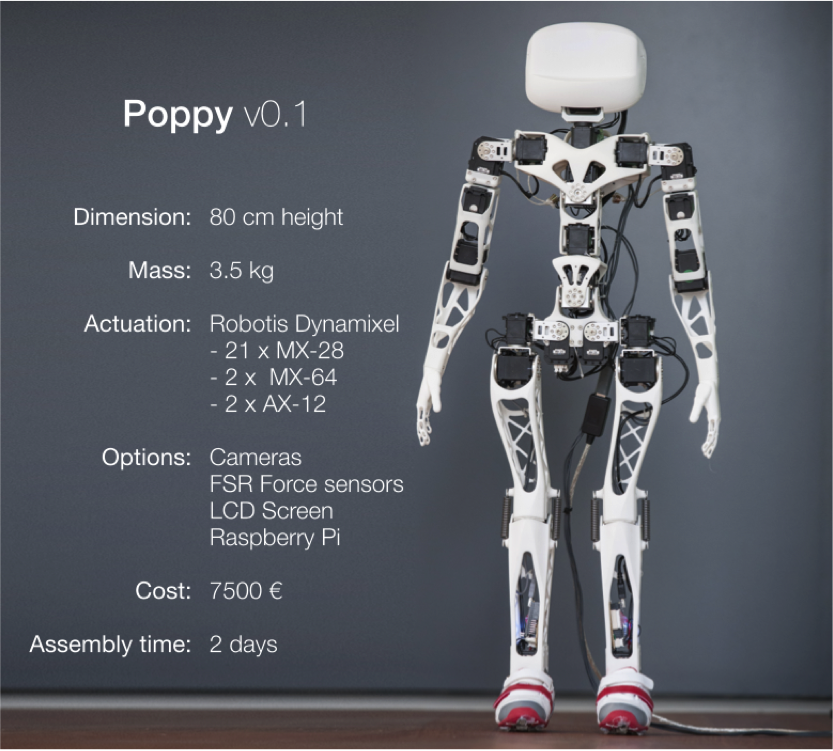
\includegraphics[width=0.9\columnwidth]{images/poppy.png}
\end{center}
}

\block{Reproductible research}{

Poppy is designed to conduct robotic experiments and integrate several key abilities in an easy-to-use robotic platform:
\begin{itemize}
    \item \textbf{Easy To Duplicate:} The overall time to assemble all mechanic components of Poppy takes about 2 days. Adding extra
sensors is simplified by the use of Arduino components.
    \item \textbf{Robustness and Lifelong Learning:} Poppy is designed to be robust to falls and to allow long experimentations (e.g. several
hours). Also, its conception prevents it from destructing itself if wrong moves occur.
    \item \textbf{Easy To Setup:} We try to keep Poppy as Plugn’Play as possible.
    \item \textbf{Affordable:} To make Poppy widely accessible, we keep the cost relatively low. You can afford all components for
7500-8000 Euros.
\end{itemize}
\vspace{1cm}
\begin{center}
    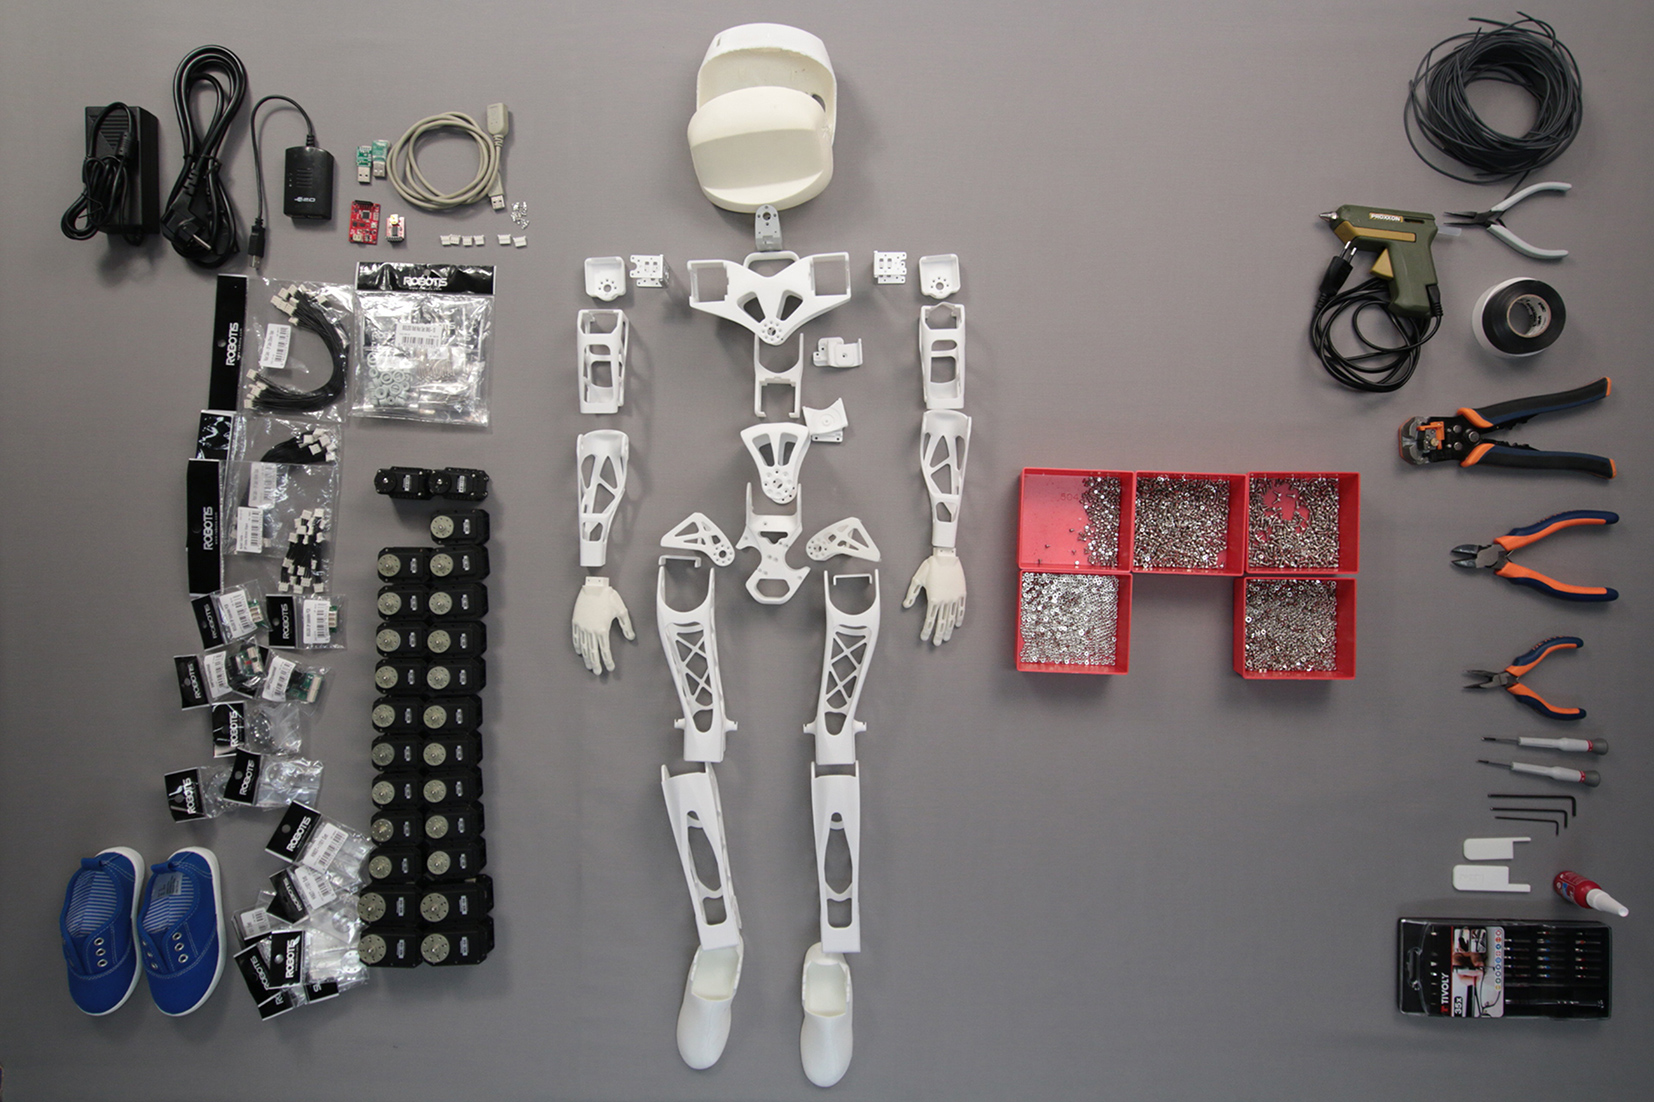
\includegraphics[width=0.9\columnwidth]{images/poppy_components.jpg}
\end{center}
}

\block{Scientific experiments} {
\vspace{1cm}
\begin{center}
    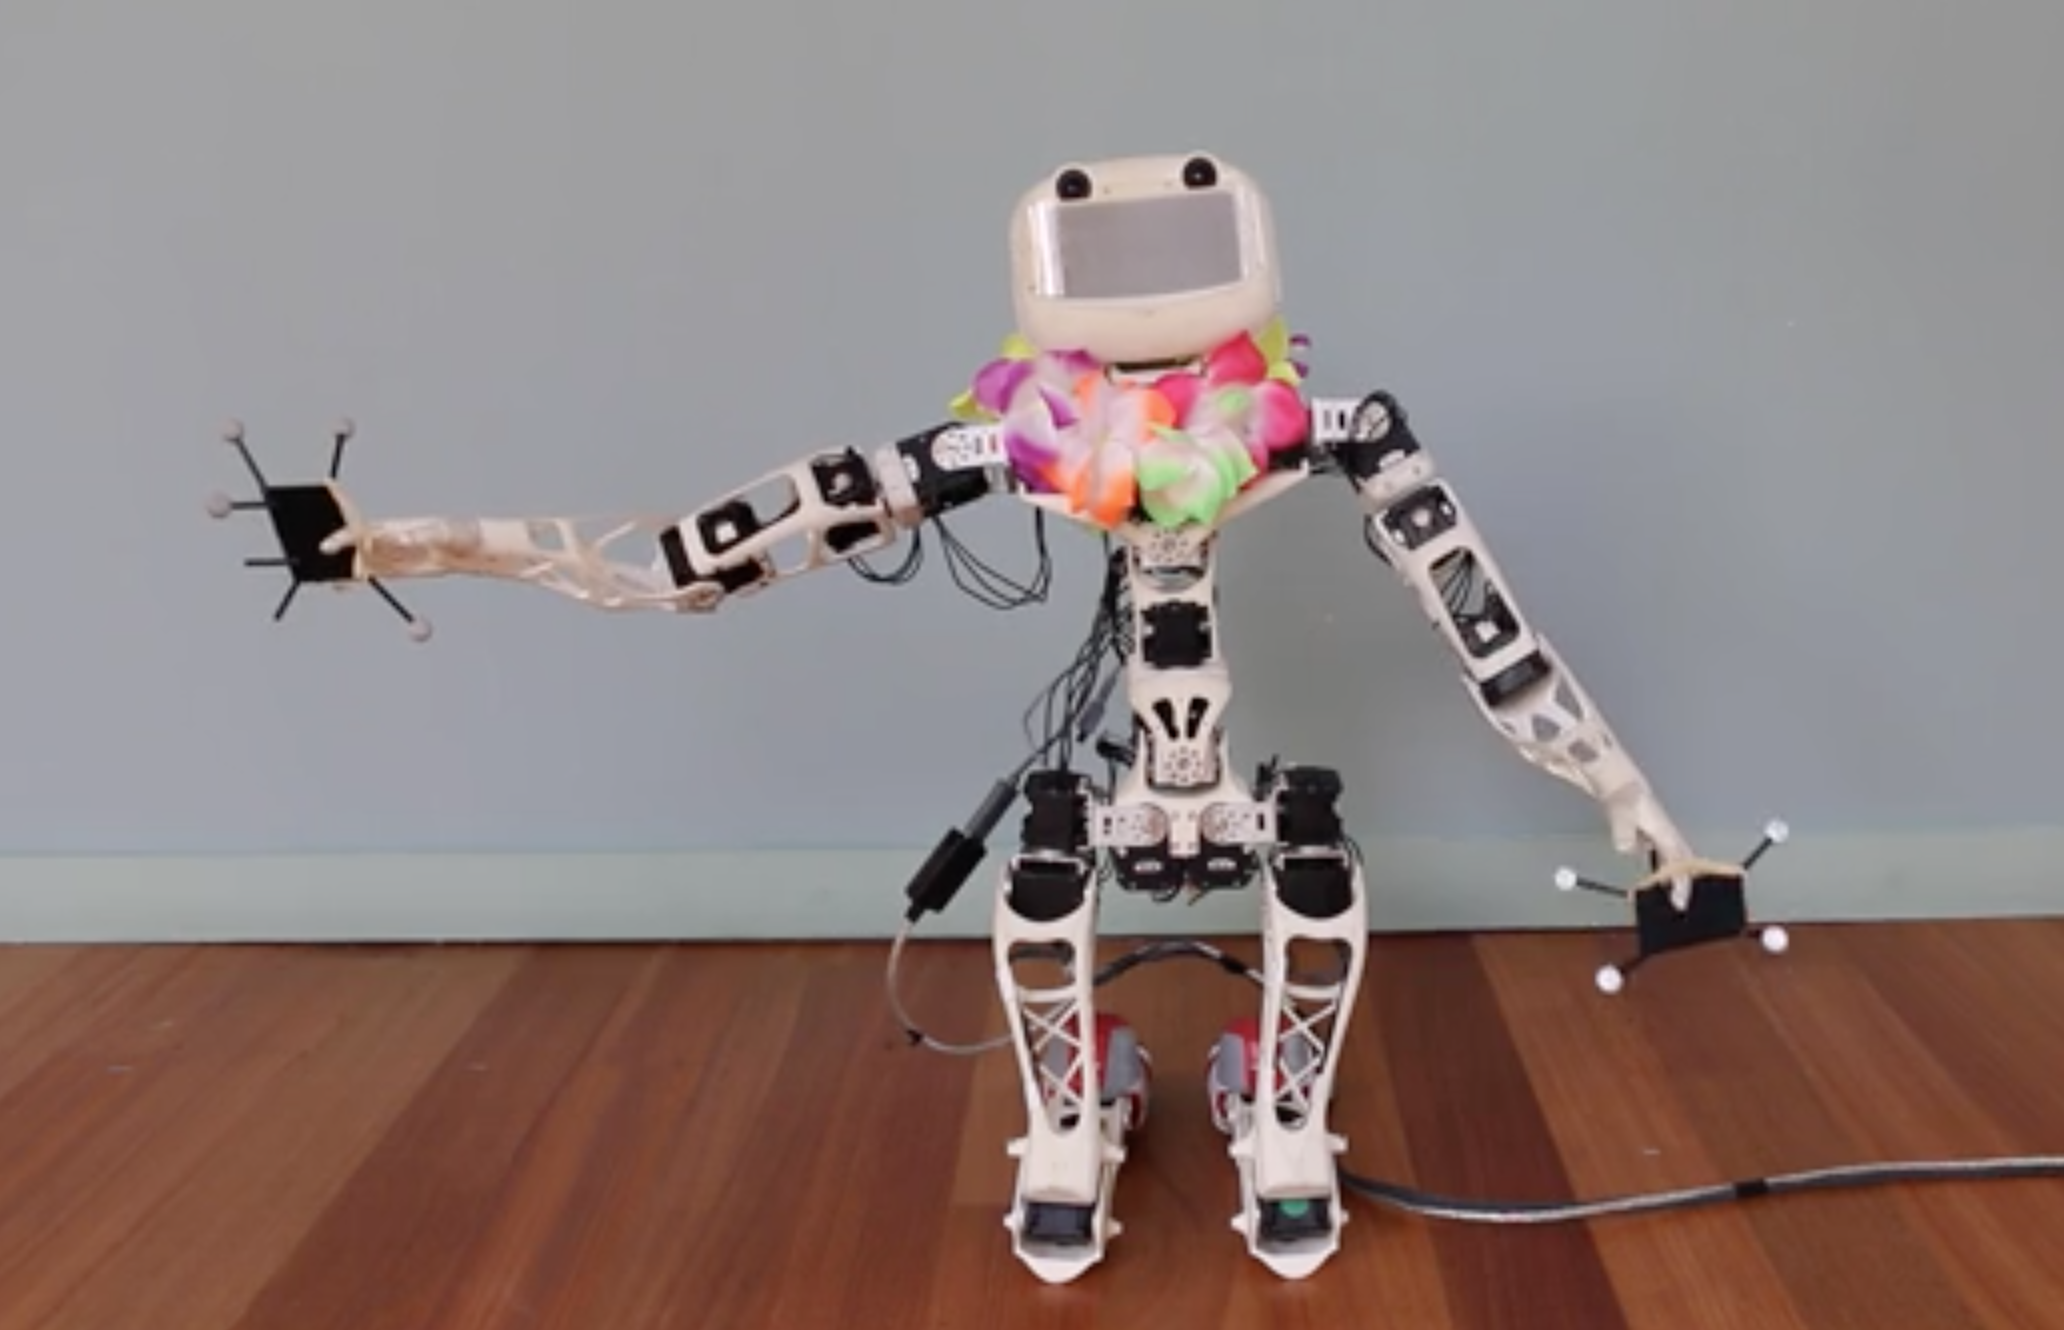
\includegraphics[width=\columnwidth]{images/poppy-explauto.png}
\end{center}
Poppy was used to compare motor versus goal babbling strategies when learning the inverse model of its arm. Thanks to the integration of pypot and explauto such an experiment can be quickly designed and realised~\cite{moulinfrier:hal-01061708}.}

\block{Artistic experiments} {
\vspace{1cm}
\begin{center}
    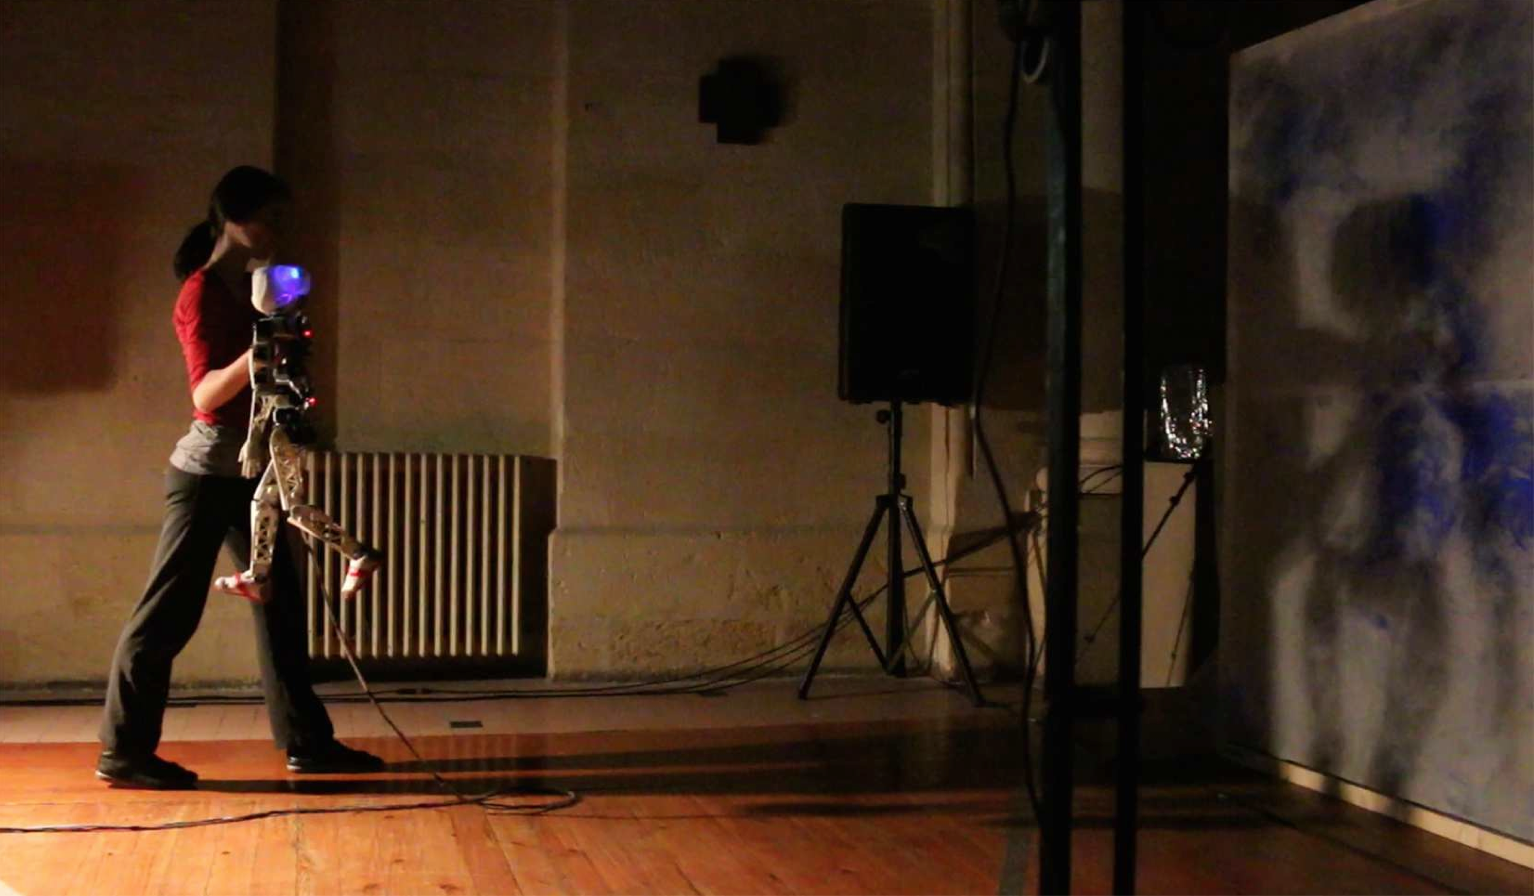
\includegraphics[width=\columnwidth]{images/poppy-stonge.png}
\end{center}
The poppy platform has also been used in artistic dance performance. 
}

\block{More information}{More information on the project can be found on our website \textbf{www.poppy-project.org}, in particular the current development of the platform is daily discussed on our forum: \textbf{forum.poppy-project.org}. Also all sources (hardware and software) of the Poppy project are distributed under open-sources licenses on our GitHub page \textbf{www.github.com/poppy-project/}.}

\block{References}
{
	% \vspace{-10pt}
	\nocite{*}
	\bibliographystyle{abbrv}
	\renewcommand{\section}[2]{}% Hack to remove bibliography title
	\bibliography{ref}
	\vspace{-10pt}
}

\end{multicols}
\vfill
\end{document}
